\section{Eigenes Modell zu CIFAR 10}

%___________________________________________________________________

\begin{frame}{Aufgabenstellung}
    \begin{itemize}
        \item \textbf{Aufgabe:} Klassifikation von CIFAR-10 Bildern
        \item \textbf{Datensatz:}
            \begin{itemize}
                \item 10 Klassen
                \item 60.000 Bilder, Größe $32\times32\times3$
                \item Trainingsset: 49.000 Bilder
                \item Validierungsset: 1.000 Bilder
                \item Testset: 10.000 Bilder
            \end{itemize}
        \item \textbf{Ziel:} Modell in \emph{maximal 10 Epochen} trainieren, um Bilder korrekt zu klassifizieren
    \end{itemize}
\end{frame}



%___________________________________________________________________

\begin{frame}{Architektur des Modells}
    \begin{figure}
        \centering
        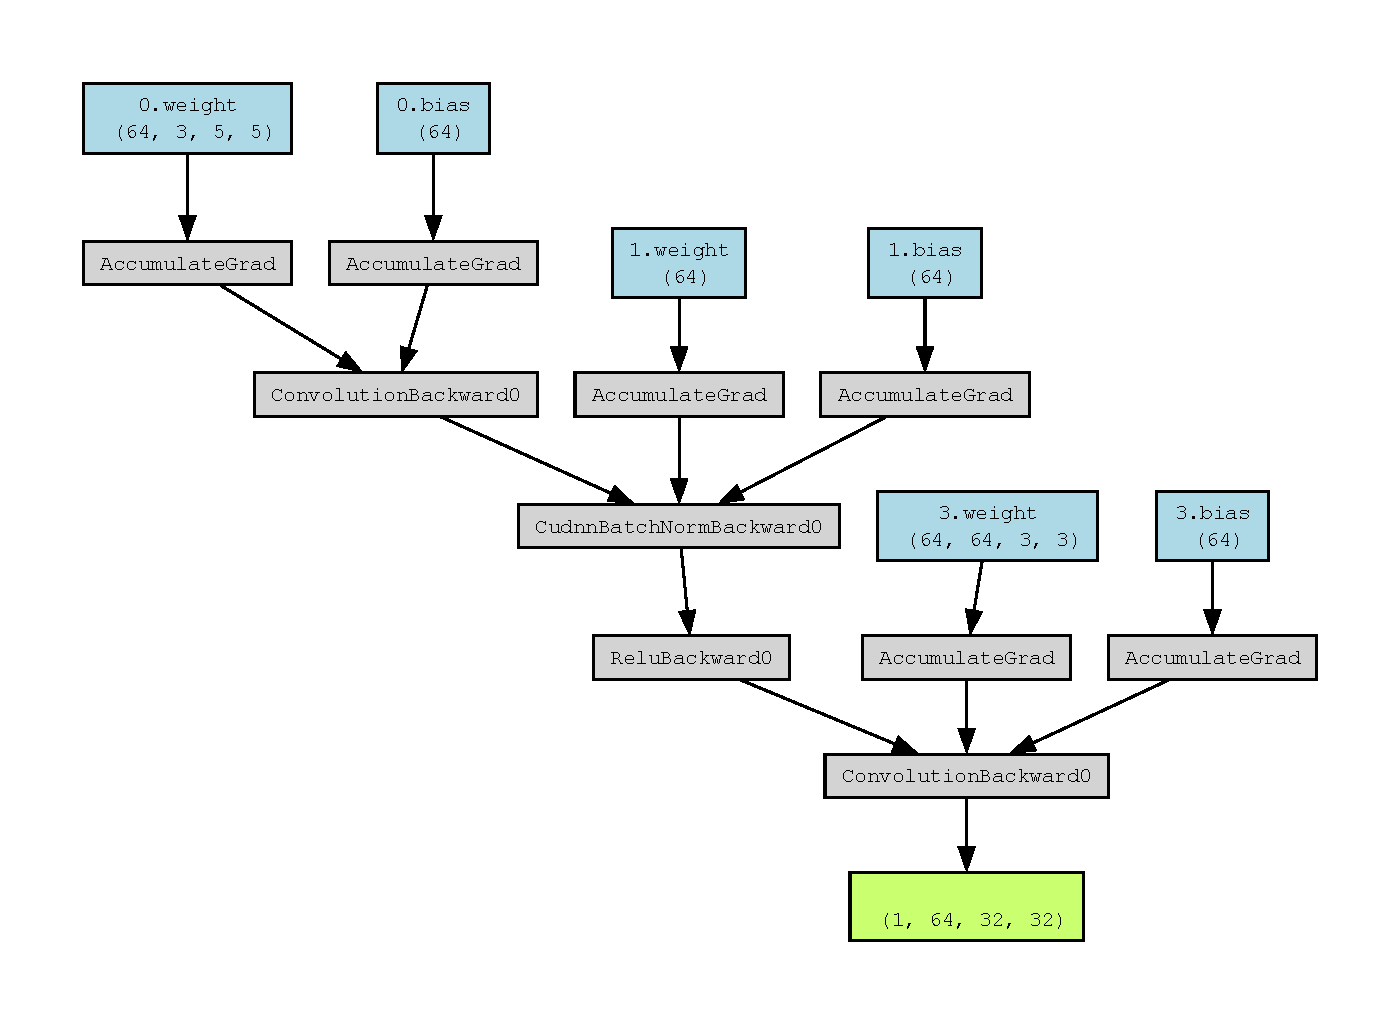
\includegraphics[width=\imagewidth, height=\imageheight, keepaspectratio]{reduced_graph.pdf}
    \end{figure}

\end{frame}

%___________________________________________________________________

\begin{frame}{Ergebnisse des besten Modells}

\begin{itemize}
    \item \textbf{Gewählte Hyperparameter:}
        \begin{itemize}
            \item ch1 = 64, ch2 = 64, ch3 = 64
            \item Lernrate = 0.00086
            \item Weight Decay = 3.81e-6
        \end{itemize}
    \item \textbf{Best Validation Accuracy:} \alert{75.70\%}
    
    \item \textbf{Trainings-Accuracy:} \alert{73\%}

    \item \textbf{Test Accuracy:} \alert{75.05\%}
\end{itemize}
\end{frame}

%___________________________________________________________________

\begin{frame}{Accuracy für verschiedene Klassen}
    \begin{figure}
        \centering
        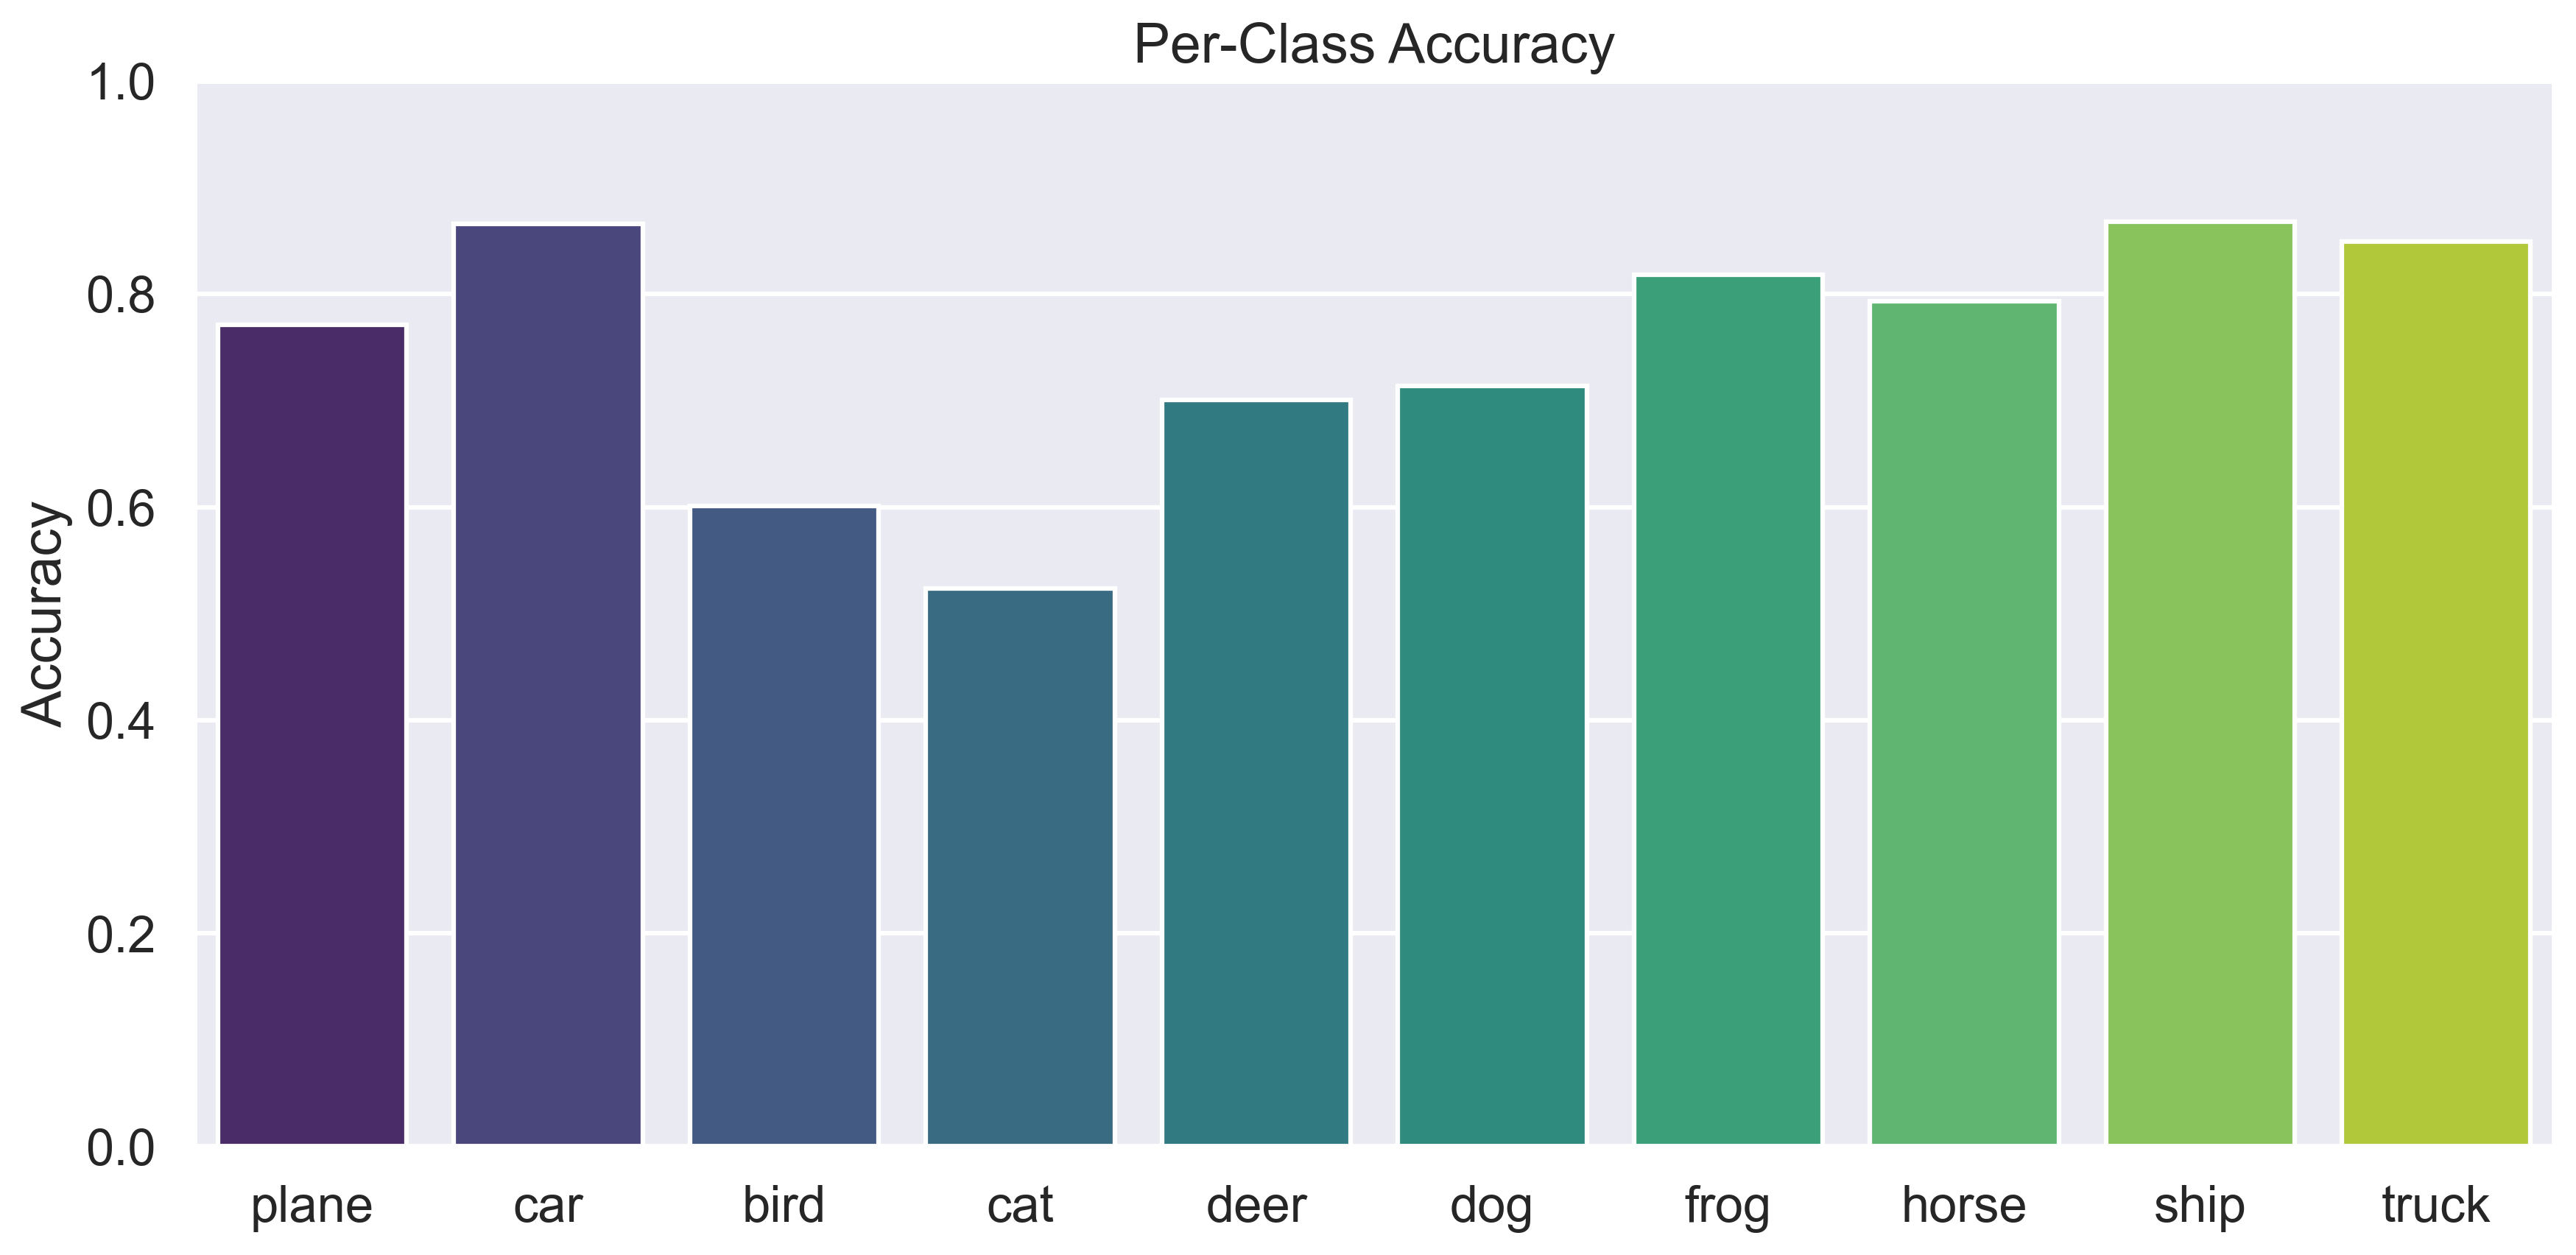
\includegraphics[width=\imagewidth, height=\imageheight, keepaspectratio]{class_accuracy.png}
    \end{figure}
\end{frame}

%___________________________________________________________________

\begin{frame}{Confusion Matrix}
    \begin{figure}
        \centering
        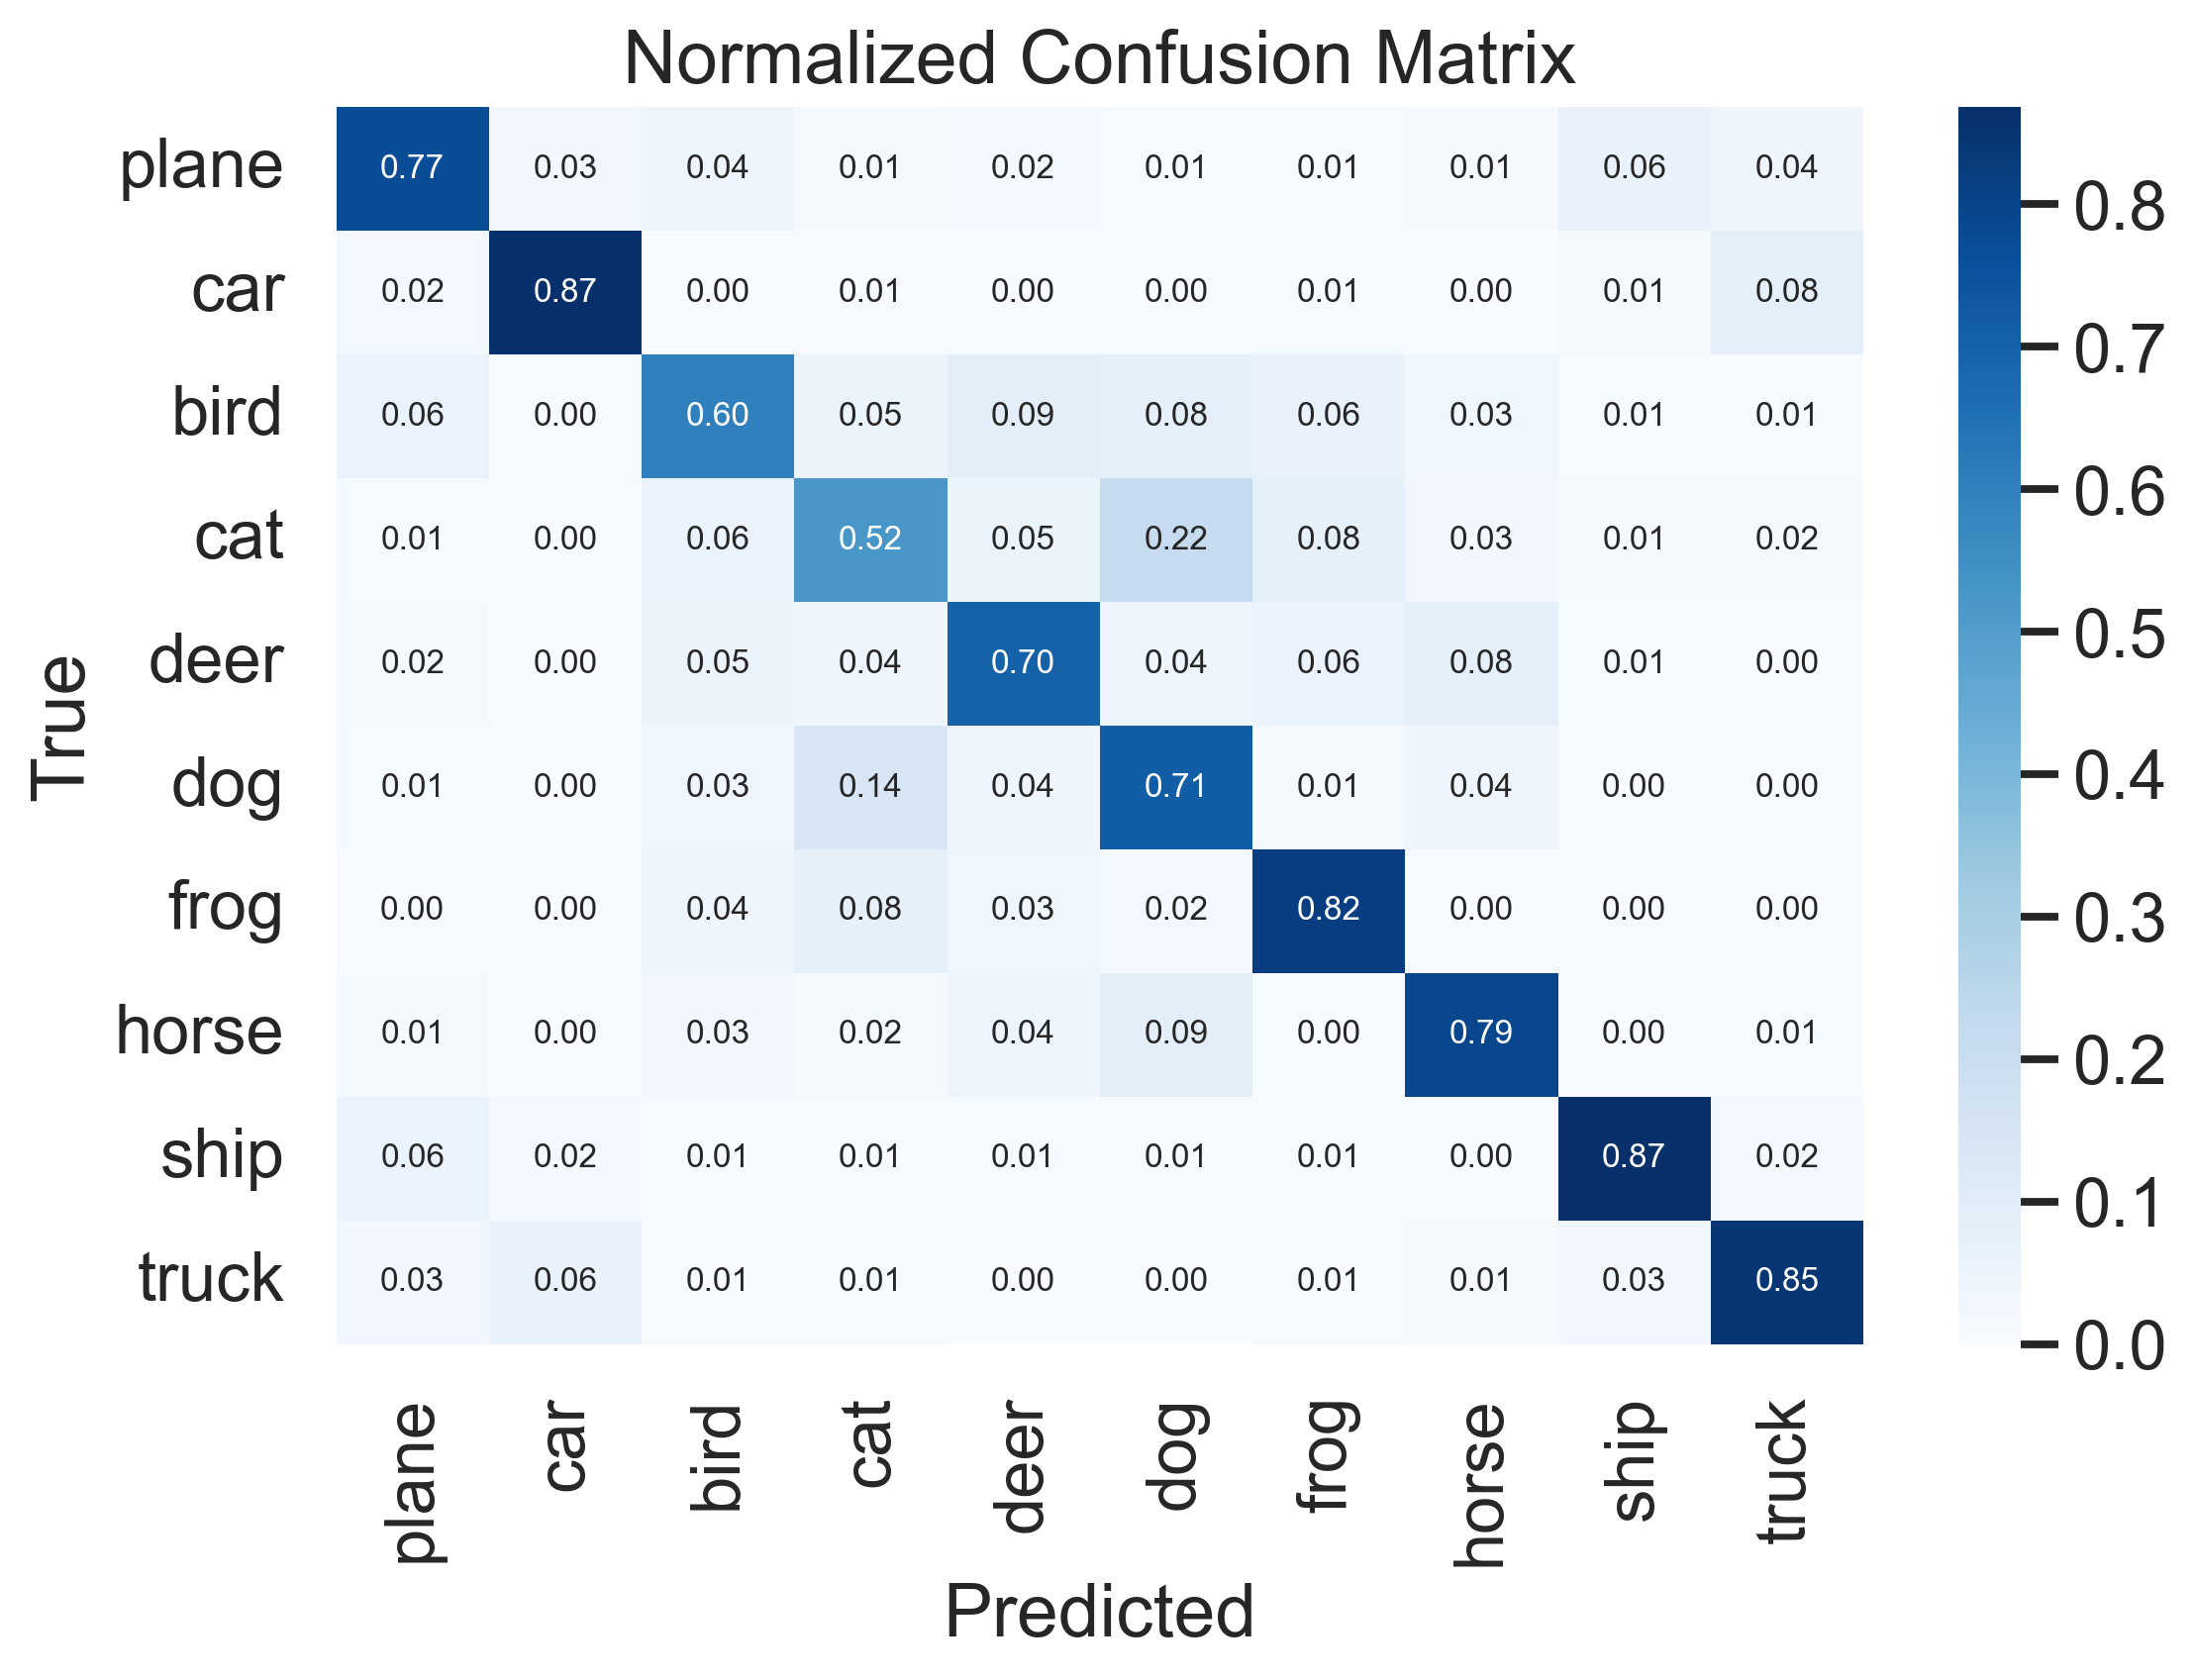
\includegraphics[width=\imagewidth, height=\imageheight, keepaspectratio]{confusion_matrix.png}
    \end{figure}
\end{frame}

%___________________________________________________________________

\begin{frame}{Beispielvorhersagen}
    \begin{figure}
        \centering
        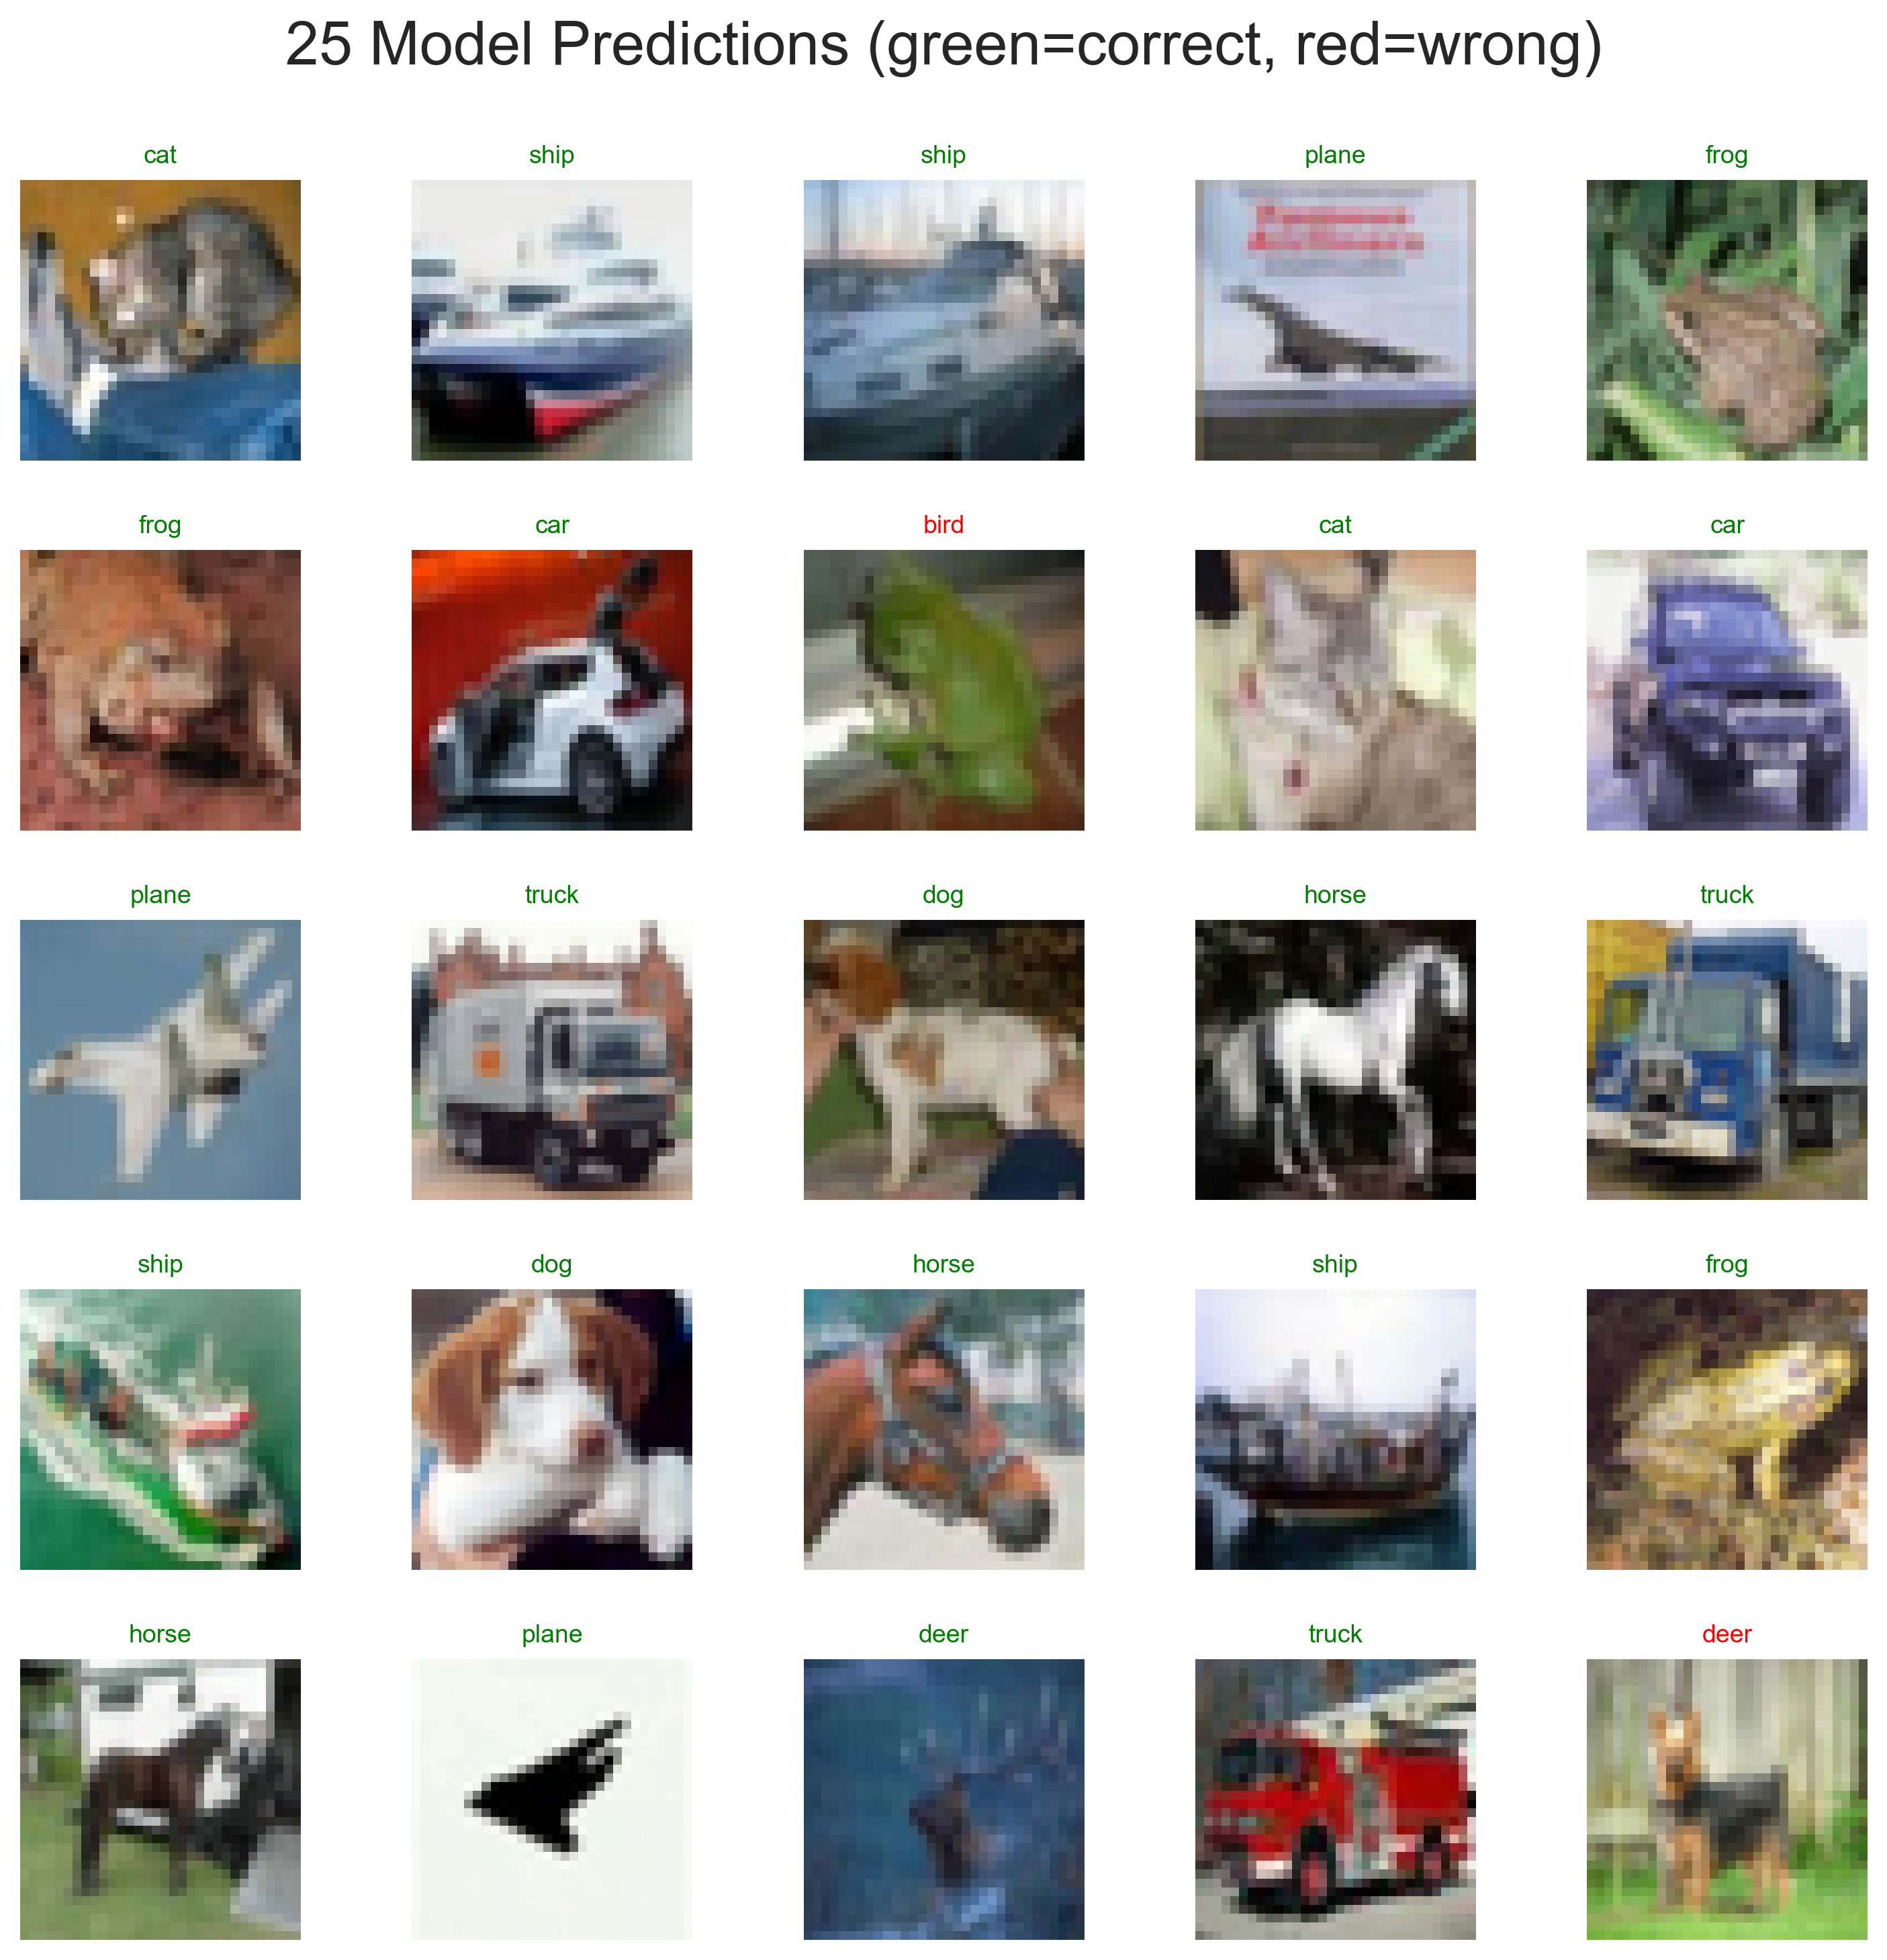
\includegraphics[width=\imagewidth, height=\imageheight, keepaspectratio]{predictions_grid.png}
    \end{figure}
\end{frame}

